\documentclass[a4paper]{article}

% Support for Norwegian letters
\usepackage[latin1]{inputenc}
\usepackage[T1]{fontenc}
\usepackage{amsmath,amsfonts,amssymb,amsthm,booktabs,array,mathtools}
% consider package mhchem for typesetting chemical formulas
\usepackage{graphicx}

% Proper space and font for integral differential term
\newcommand{\dd}{\; \mathrm{d}} 
% Shorcut for ODEs with proper font
\newcommand{\diff}[2]{\frac{\mathrm{d} #1}{\mathrm{d} #2}}
% Shortcut for PDEs with proper font (shortcut: PDB)
\newcommand{\pdiff}[2]{\frac{\partial #1}{\partial #2}}
\newcommand{\pdiffn}[3]{\frac{\partial^{#3} #1}{\partial #2^{#3}}}

% Absolute value and norm commands.
% Read the mathtools.pdf to fix these!
\providecommand{\abs}[1]{\lvert#1\rvert} 
\providecommand{\norm}[1]{\lVert#1\rVert}

\title{Polyadenylation in different cellular compartments}

% Set the depth of section numbering
\setcounter{secnumdepth}{0}

\begin{document} 

\maketitle

\subsection{Introduction}
In eukaryotes polyadenylation occurs after 3' cleavage as one
of the last stages of pre-mRNA processing. The cleavage/polyadenylation process
is triggered by the polyadenylation signal (PAS) which is typically found 10-30
nucleotides downsteam the cleavage site. More generally, adenylation of RNA is
found in nearly all kingdoms of life, but plays opposite roles in bacteria and
eukaryotes, where in bacteria adenylation promotes degradation of RNA, while in
eukaryotes an RNA's poly(A) tail protects from degradation.

We investigated the RNA-seq data for 5 GENC ODE cell lines for signs of
polyadenylation by trimming and remapping those reads that were originally
unmappable and ended in a stretch of As or beginning with a stretch of Ts. We
subsequently merged the polyadenylation sites into clusters in a similar way to
Tian et. al \cite{tian_large-scale_2005}. In total, for all cell lines and
compartments, we obtained 29860 putative polyadenylation sites. A putative
polyadenylation site is here defined as a site at which two or more trimmed
reads cluster together, or a site at which a read lands at a previously
annotated polyadenylation site. Annotated polyadenylation sites were found by
merging and clustered 43187 sites from the polyAdb \cite{park_design_2007} with
35791 sites from GENCODE to obtain a total of 50696 annotated polyA sites.
16657 of our polyA sites fall at annotated ones (81\% or 13517 of these are in
3UTRs), leaving a total of 13203 putative novel polyadenylation sites in the
genome (Fig \ref{fig:Venn}

\begin{figure}[h]
	\centering
		\includegraphics[scale=0.5]{../Figures/genome_venn_diagram.eps}
	\caption{Overlap between identified poly(A) sites and two annotations}
	\label{fig:Venn}
\end{figure}
\subsection{Polyadenylation in the nucleus and in the cytoplasm}

The RNA-seq protocol for the Gingeras data is not optimized for 3' ends,
therefore we expected to find most poly(A) sites for transcripts with high RPKM. To
investigate this, we calculated the ratio of discovered to annotated poly(A) sites
in 3UTRs that do not overlap any other genomic feature. Figure \ref{fig:RPKM}
shows the relationship between RPKM and poly(A) discovery ratio for annotated
3UTRs. As can be seen, there is a positive association between RPKM and
poly(A) discovery (r = 0.52, p < $10^{-10}$), however there is considerable
variation even for high RPKM transcripts. The average number of poly(A) sites
found per 3UTR was 1.7, and the average ratio of poly(A) sites to annotated was
0.9. That fewer than 1 per annotated site are found probably reflects both that
the method is not exhaustive, and that not all annotated poly(A) sites are in
use at a given time.

\begin{figure}[h]
	\centering
		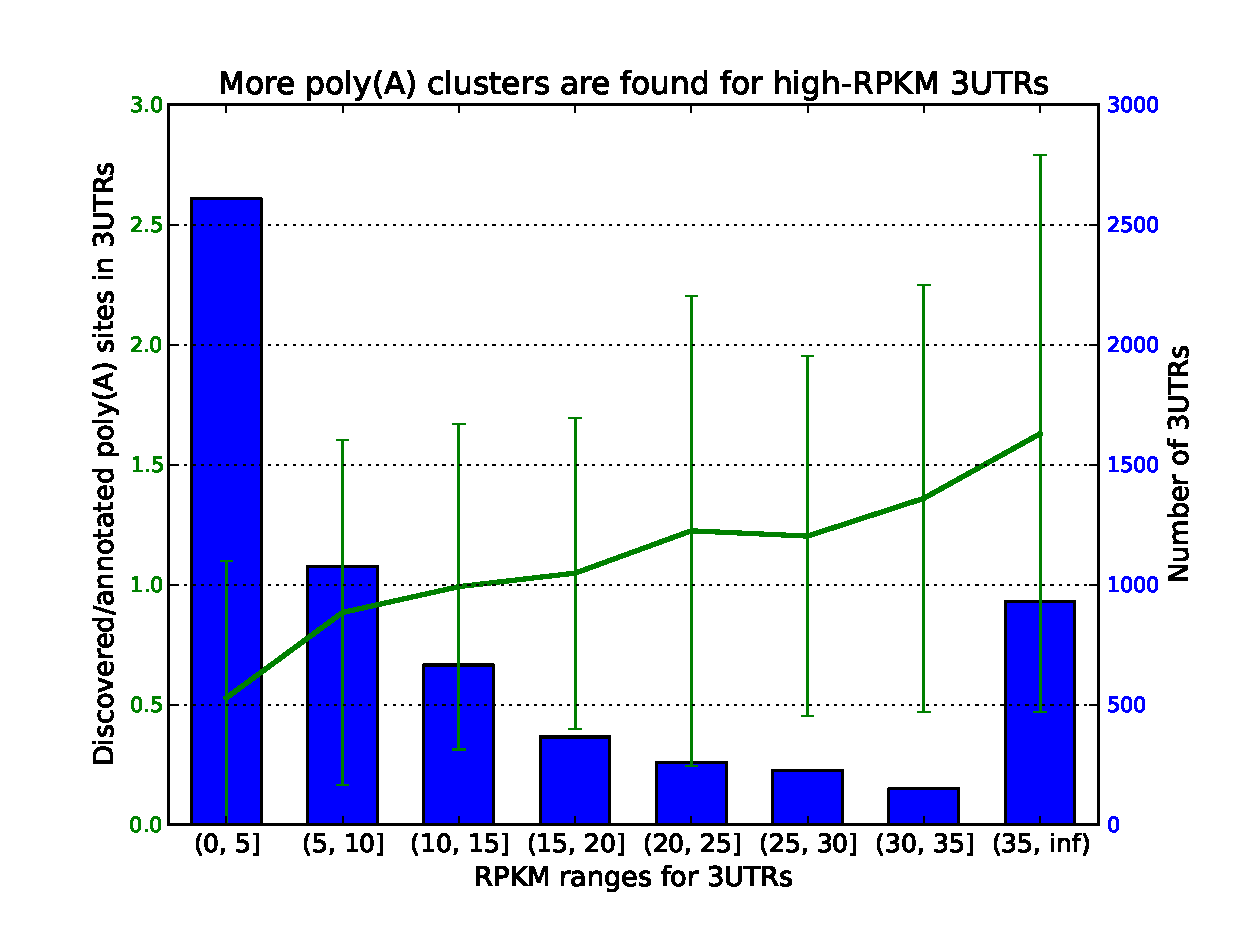
\includegraphics[scale=0.5]{../Figures/More_polyA_clusters_for_high_RPKM_3UTRS.eps}
	\caption{RPKM-poly(A) discovery link}
	\label{fig:RPKM}
\end{figure}
\subsection{Polyadenylation in the nucleus and in the cytoplasm}

We merged the poly(A) sites from 5 cell lines in the nucleus and cytoplasm
separately for the poly(A)+ and poly(A)- fractions and compared the
distribution of the polyadenylation sites in the genome (Figure
\ref{fig:region_counts}). The difference between poly(A)+ and poly(A)-
fractions is that a poly(A) filtering step in the sample preparation protocol
assigns RNA with a poly(A) tail on average longer than 30nt to the poly(A)+
fraction, and the remainder goes to the poly(A)- fraction.

\begin{figure}[h]
	\centering
		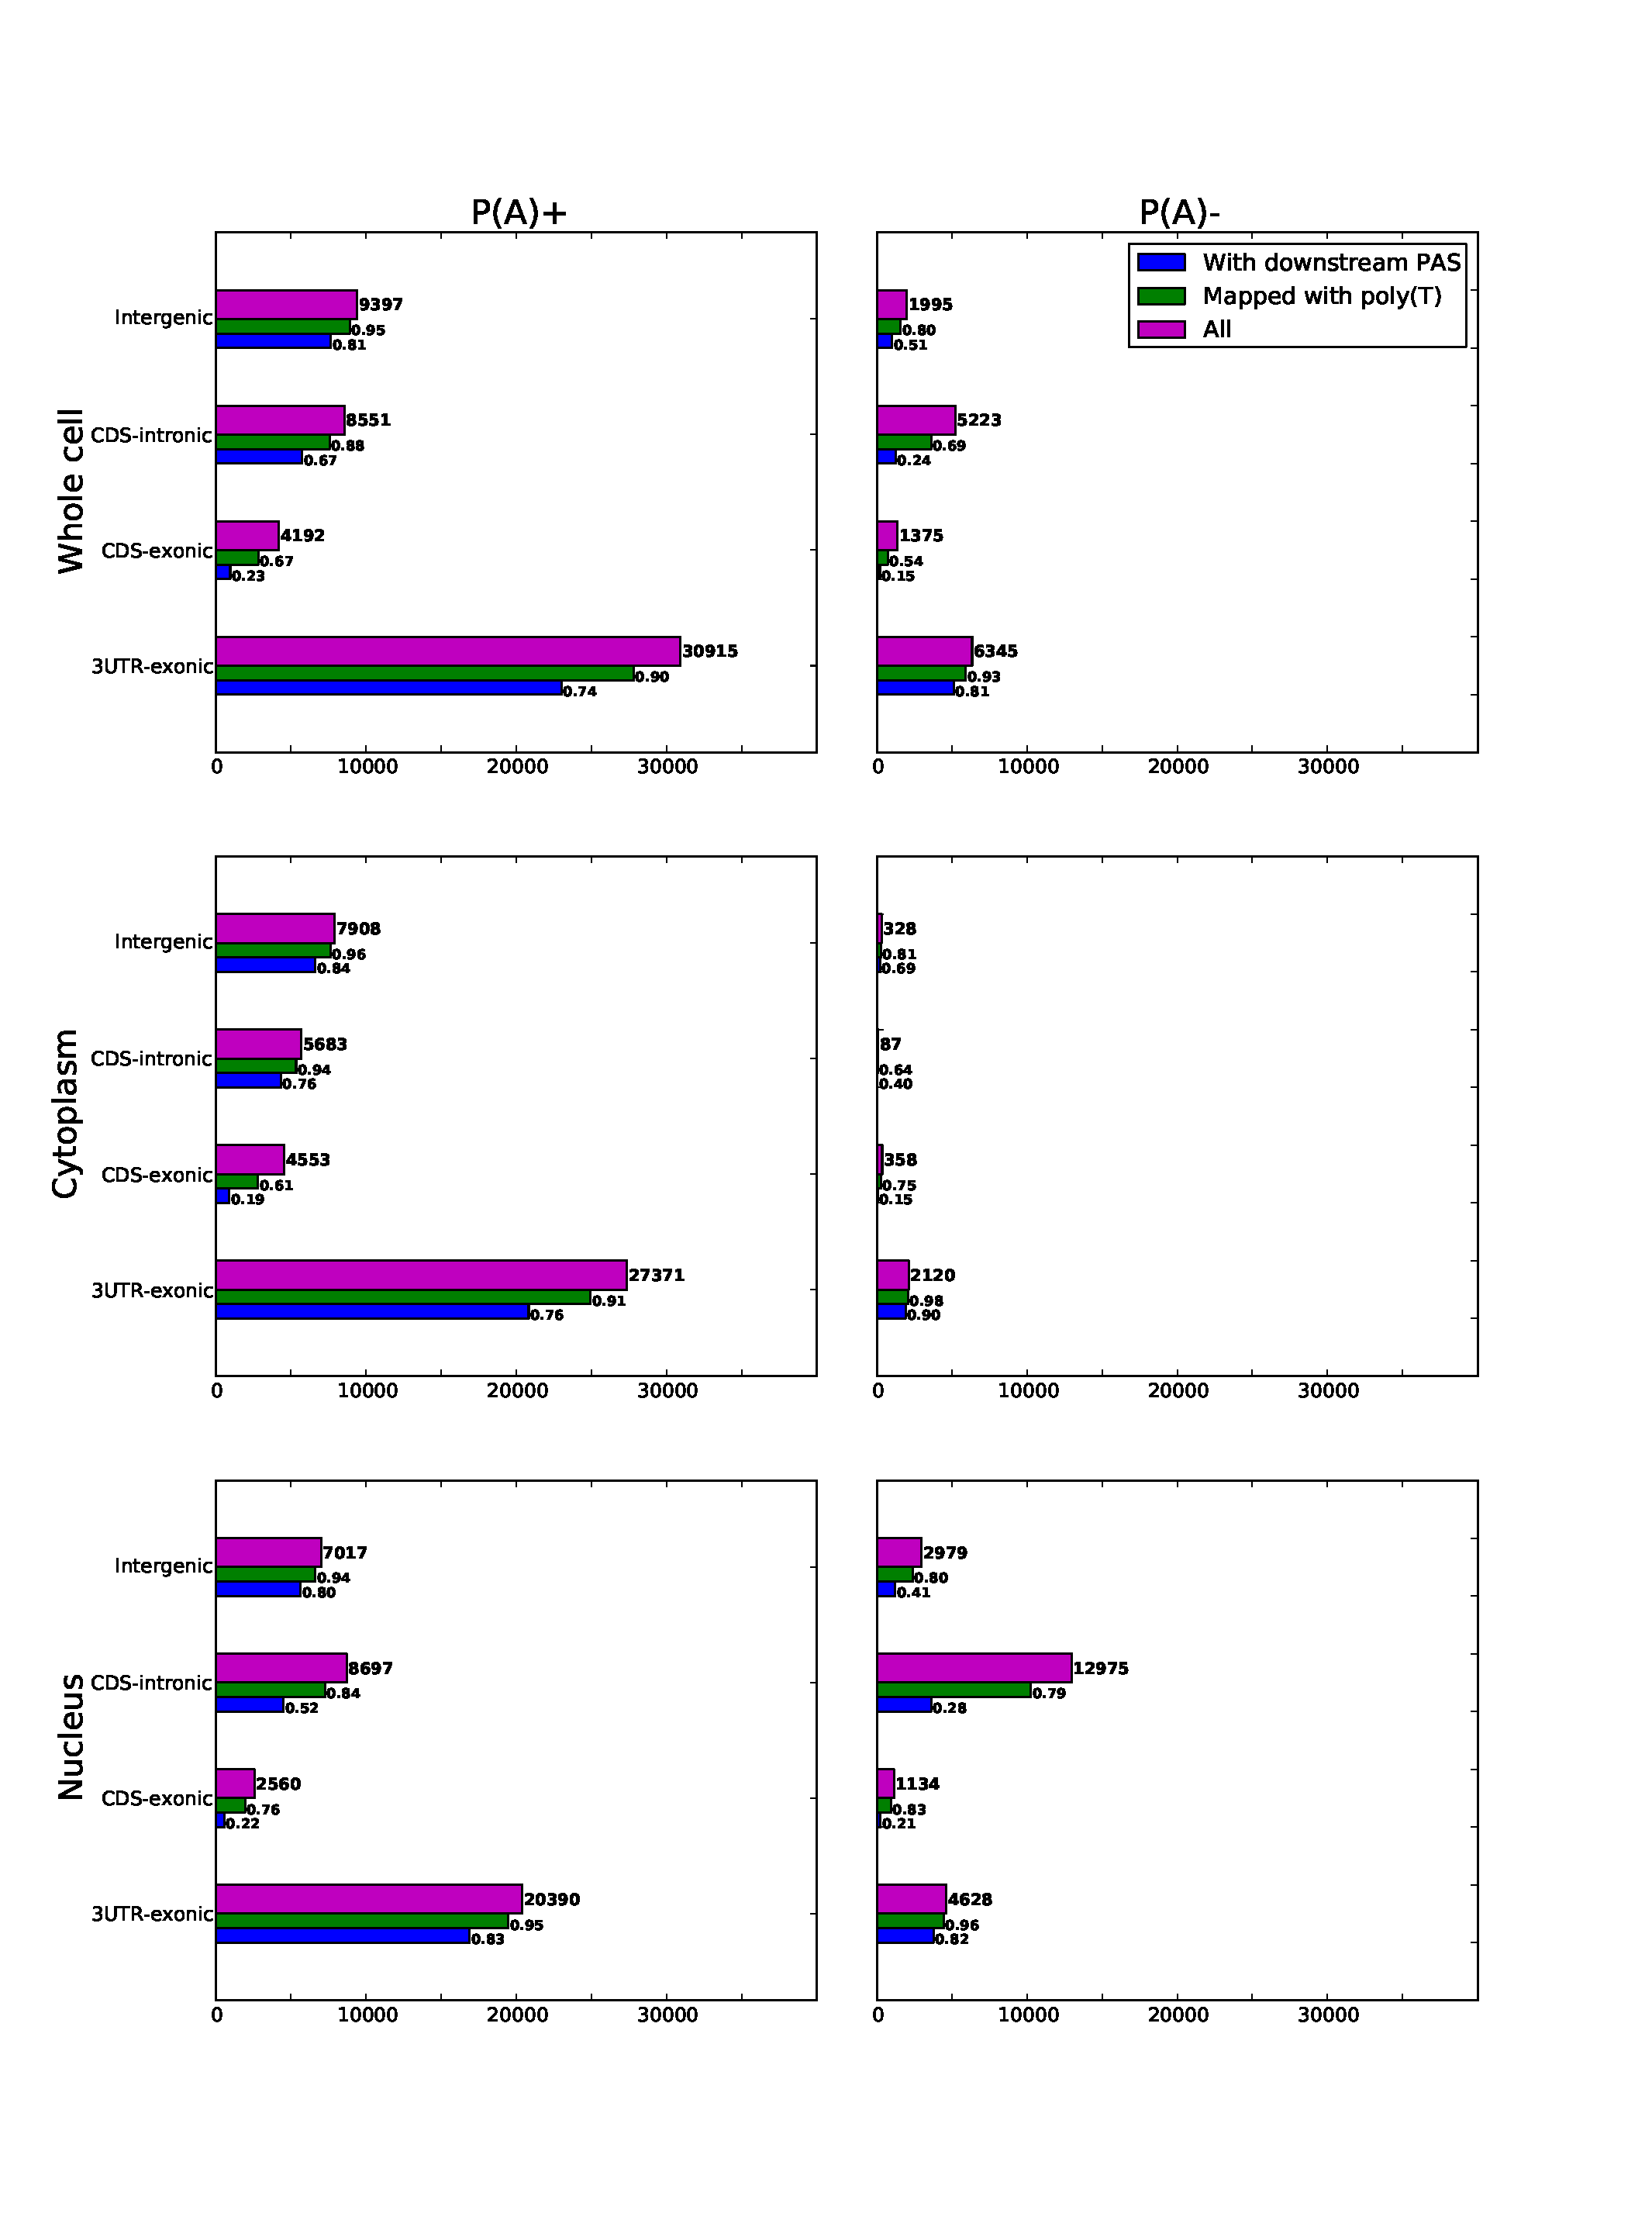
\includegraphics[scale=0.50]{../Figures/nr_of_polyA_different_compartments_non_stranded_ABRIDGED_2+}
	\caption{Polyadenylation marks in different cellular compartments, in
	different genomic regions, for both poly(A)+ and poly(A)- fractions}
	\label{fig:region_counts}
\end{figure}
\subsubsection{Number of polyadenylatoin events in poly(A)+ fraction}
Polyadenylation reads from the poly(A)+ were remarkably evenly distributed in
the genome in the whole cell, cytoplasm, and nucleus (Figure
\ref{fig:region_counts}). Whole cell and cytoplasm have nearly the same number
of polyadenylation clusters, and the relative distribution of clusters in the
different genomic regions is almost the same, with 3UTR-exonic having clearly
the most. The 3UTR in whole cell, cytoplasm have, respectively, XXX, XXX, XXX
sites, which make up roughly 60\% of the total polyadenylation
sites. The blue bar in Figure \ref{fig:region_counts} shows the percentage of
clusters that have one of the 8 indentified PAS \cite{} within 40nt downstream
the polyadenylation site. In the 3UTR, 87\% of clusters are associated with a
PAS site, and of these similar to 85\% that was found in a study using EST data
\cite{}.

% NOTE that 85% is not true. The figure is 75% for AATAAA + ATTAAA In your
% summary output with the tail and everythig you need to specify the good pas.
% Tian found 70% of the two, and bauding 75 %.  TODO this T PAS ratio things
% for all, to estimate the 'degree' (not number) of genuine non-PAS related
% polyadenylation

By comparing the whole cell data with the  nucleic
and cytoplasmic compartments in Figure \ref{fig:region_counts}, it is clear
that the distribution of poly(A) reads in the genome is similar for the
poly(A)+ fraction.

%# NOTE you are rewriting from here.
%# IDEA: is it possible that noise is A-tail favored? That would explain the
%results in 1-size clusters. It's odd but in the 1-clusters, the pa(A)-
%fraction has more annotated than the pa(A)+ one.
% TODO! Include a figure from the genome browser with poly(A) reads!!!!!! super
% easy and super good.

fractions From Figure , it can be seen that there are found
proportionally a larger fraction of poly(A)- reads in the nucleus than in the
cytoplasm. The polyadenylation marks in the cytoplasmic poly(A)- fraction can
come from mRNA that is being degraded (as the poly(A) tail is gradually
decreased in length before degradation), which will be discussed below.

%We wanted to compare poly(A) sites in the nucleus and cytoplasm for different
%genomic regions. While poly(A) sites in the cytoplasm are expected to derive
%from from the 3' ends of stable, multi-copy mRNA, the poly(A) sites from the
%nucleus are expected to stem from mRNA diffusing toward the cytoplasm, mRNA
%undergoing processing, and possibly some RNA undergoing degradation
%\cite{shcherbik_polyadenylation_2010,slomovic_addition_2010}.

As can be seen, the nuclear regions capture polyadenylation signals both in the
poly(A)+ and poly(A)- fractions in the intronic regions. Intronic
polyadenylation has been identified for many genes \cite{tian_widespread_2007},
which could explain that markers of polyadenylation is found in the poly(A)+
fraction.  However, it was unexpected to find polyadenylation markers in the
poly(A)- fraction. Their presence in this fractions means that they originate
from RNA that had a poly(A) tail of 30nt or less. This could be the
evidence of a different type of adenylated RNA in the nucleus, such adenylation
as a marker for degradation \cite{slomovic_addition_2010}

It can be seen that for the poly(A)+ fraction the whole-cell samples are most
similar to the cytoplasmic ones. However, while the over-all numbers are lower for
the nucleus compared to the cytoplasm and whole cell, the relative distribution of
poly(A) reads in the different genomic regions is the same. This could indicate that
previous studies of polyadenylation that have used whole cell extracts and
poly(A)+ fractions have given conclusions that are representative for both the
cytoplasm and the nucleus.

In the poly(A)- fraction it can be seen that it is the nucleus that has more
marks of polyadenylation than the cytoplasm. In other words, it seems that
there is more adenylation with short poly(A) tails in the nucleus compared to
the cytoplasm. For some of the adenylation sites in the 3UTR this difference
could be explained by polyadenylation caught-in-action, however it does not
explain the increase in the other genomic reagions.

To verify that the T-mapped reads give use the orientation of the transcript,
we checked for poly(A) sites in a strand-specific non-overlapping set of GENCO
DE 3UTRs. As can be seen in figure X, by using the T/A tail and +/- mapping we
get strand specific bla bla % TODO
%To investigate whether the markers of polyadenylation we observe are in the
%sense or anti-sense direction to anntated genomic features, we looked at only
%those genomic regions that have features in one sense uniquely, and that do not
%overlap with any other genomic features. Figure \ref{fig:sense} shows this.
%%\begin{figure}[h]
	%%\centering
		%%\includegraphics[scale=0.34]{../Figures/sense_strand_percentages}
	%%\caption{Sense strand mapping percentages in different cellular compartments, in
	%%different genomic regions, for both poly(A)+ and poly(A)- fractions}
	%%\label{fig:sense}
%\end{figure}
%For 3UTR-exonic regions, more than $90\%$ of the poly(A) sites are mapped to the
%annotated strand. TODO doublecheck the non_stranded regions and re-run this
%simulation for better results!

Given the recent reports of degradation-related adenylation in humans, we
looked for signatures of degradation. Marks of adenlyated assisted degradation
can be expected to be less reproducable and less location-specific than 3' mRNA
polyadenylation, although in \cite{} the adenylation sites were frequently
found at identical or close-by locations both in the nucleus and in the
cytoplasm. Any degrdation-related adenylation site would not be likely to
contain the PAS-signal downstream, which 85\% of annotated polyadenylation
sites in 3UTRs do (Table 1). Thus we searched for adenylation sites that were
not at annotated sites and that did not contain one of the PAS downstream.
Since degradation-related (A)-tails are shorter than the ones found at the 3'
end of mRNAs, these tails are expected to be represented with reads from the 3'
pair-end read, thus being originally found with a poly(T) header. Further, as
well as genuine poly(A) signals, they are expected to map to the sense strand.
Table XXX contains an overview of all polyadenylation sites without PAS. As can
be seen $\dots$. Is the increase in poly(A)- adenylation in the nucleus to the
cytoplasm due to non-PAS adenylation for all regions? Would be great. Yes! You
see it. It's not a very string signal, but both the T/A ratio and the non-PAS
ratio increases between poly(A)- nucleus and cytoplasm.

Given the possibility of non-PAS adenylation in the human genome, we decided to
search for it. Assuming that all reads from 'T' For all the poly(A) clusters we found, we calculated the non-PAS
clusters to PAS-clusters (from T-based clusters). Figure X compares cytoplasmic
and nucleuc poly(A) minus. As can be seen $\ldots$

Nucleus: out of clusters with 2 or more:

Total 3777. With Ts: 2417- 700 (annotated + PAS)

Further: this definitely holds true if we look at the clusters with only 1
coverage! Here there are 23k Ts and 11kAs for NucleusMinus, while Cytoplasm has
got 3.5k to 3.7k. Next question is, where do they come from? What genomic
region?

obvious follow-up question is then: where do they land? In what types of
transcript do they land? coding? noncoding? blablu blibli? Maybe use Andrea's
index of gencode 7 for finding out where they land?

Also, the sense/antisense strand would be nice too. Then you have to fix all
that.
The

% too much work with the table in latex. make it easier. maybe you can make the
% final table this way.
%\input{table1}

%1 TODO make the big table you mention about in the first part
%2 TODO make the unique sense-antisense libraries and make sure they don't
%overlap each other. Return similar values as for polyadenylation, but now
%include K562 nucleoplasm and chromatin as well (actually you can include them
%in the above too).

DISCUSSION

\begin{enumerate}
	\item It's possible to use conventional RNA-seq to study polyadenylation,
		you just need a lot of reads
	\item Evidence for geniune poly(A) reads lie in the strandedness of the
		reads and the A/T origin of the reads. Long tails may have A-endings,
		but probably few, while short A-tails are expected to have only Ts.
	\item Difference in nucleus/cytoplasm for poly(A)+/-, maybe due to
		degradation-related adenylation? 

\end{enumerate}

\bibliographystyle{plain}
\bibliography{/users/rg/jskancke/phdproject/bibtex/jorgsk}
%\bibliography{/home/jorgsk/work/bibtex/jorgsk}

\end{document}


